\documentclass[12pt]{article}


\usepackage[margin=1in]{geometry}
\usepackage{amsmath}
\usepackage{amsfonts}
\usepackage{graphicx}      % include this line if your document contains figures
\usepackage{enumerate}
\usepackage{cite}
\usepackage{circuitikz}
\usetikzlibrary{patterns}
\usetikzlibrary{shapes.geometric}


\definecolor{msblue}{rgb}{0.357, 0.608, 0.835}
\definecolor{msgreen}{rgb}{0.439, 0.678, 0.278}
\definecolor{msred}{rgb}{0.753, 0, 0}
\definecolor{msyellow}{rgb}{0.984, 0.737, 0.0196}



\title{Figures for Unit 2 - Intro to Control}
\date{\today}
\author{Arne Dankers}


\begin{document}
\maketitle


\begin{figure}[htp]
    \begin{tikzpicture}
        \node[rectangle,draw,minimum size=2cm] (M1) at (0,0) {$m$};
        \node (Fa) at (3,0){$F_a$};
        \node (Fd) at (-3,0.5) {$F_d$};
        \node (Ff) at (-3,-0.5) {$F_f$};
        \node (Fg) at (0,-3) {$F_g$};
        \node (Fn) at (0,3) {$F_n$};

        \draw[->] (M1.east) -- (Fa);
        \draw[->] ($(M1.west)-(0,0.5)$) -- (Ff);
        \draw[->] ($(M1.west)+(0,0.5)$) -- (Fd);
        \draw[->] (M1.south) -- (Fg);
        \draw[->] (M1.north) -- (Fn);

    \end{tikzpicture}
\end{figure}




\begin{figure}[htb]
    \begin{circuitikz}
        \draw[fill=gray!40] (0,0) rectangle (3,3);
        \draw (0.5,3) to[spring,l=$k$] (0.5,5);
        \draw (1.5,3) to[damper,l_=$b$] (1.5,5);
        \draw[fill=gray!40] (0,5) rectangle (3,8);
        \node at (1.5,6.5) {$m$};
        \draw[thick, ->] (2.5,3) -- (2.5,5);
        \node at (2.75,4) {$F$};
        \draw[fill=gray] (1.5,1.5) circle (0.75);
        \draw (1.5,1.5) circle (5);
    \end{circuitikz}
\end{figure}


\begin{figure}[htp]
    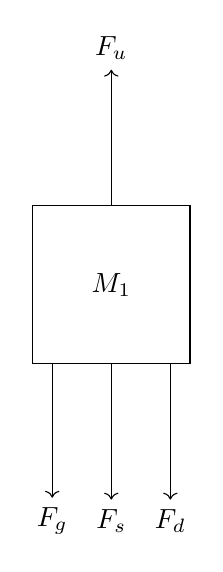
\begin{tikzpicture}
        \node[rectangle,draw,minimum size=2cm] (M1) at (0,0) {$M_1$};
        \node (Fu) at (0,3){$F_u$};
        \node (Fd) at (0.75,-3) {$F_d$};
        \node (Fg) at (-0.75,-3) {$F_g$};
        \node (Fs) at (0,-3) {$F_s$};

        \draw[->] (M1.north) -- (Fu);
        \draw[->] ($(M1.south)-(0.75,0)$) -- (Fg);
        \draw[->] ($(M1.south)+(0.75,0)$) -- (Fd);
        \draw[->] (M1.south) -- (Fs);

    \end{tikzpicture}
\end{figure}



\begin{figure}[htb]

\end{figure}
    \begin{tikzpicture}
        \node[circle,draw,minimum size=1cm] (sum_r) at (0,0) {};
        \node[rectangle,draw,minimum width=2cm,minimum height=1cm] (K) at (3,0) {$K$};
        \node[circle,draw,minimum size=1cm] (sum_d) at (6,0) {};
        \node[rectangle,draw,minimum width=2cm,minimum height=1cm] (P) at (9,0) {$P$};
        \node[circle,draw,minimum size=1cm] (sum_n) at (12,0) {};
        \node (r) at (-2,0) {$r$};
        \node (d) at (6,2) {$d$};
        \node (n) at (12,2) {$n$};

        \draw[->] (sum_r) -- node[above] {$\varepsilon$} (K);
        \draw[->] (K) -- (sum_d);
        \draw[->] (sum_d) -- node[above] {$u$} (P);
        \draw[->] (P) -- (sum_n);
        \draw[->] (sum_n) -- node[above] {$y$} ++(1,0) -- ++(0,-2) -- (0,-2) -- (sum_r);
        
        \draw[->] (r) -- (sum_r);
        \draw[->] (d) -- (sum_d);
        \draw[->] (n) -- (sum_n);

    \end{tikzpicture}
\end{document}